\chapter{Related Work}
\label{chap:related_work}

In this section we are going to provide and introduce the most recent projects and research that shed light on the integration of the three domains. However we are not going to only look on similar architecture but also we will see some similar use cases of real time face detection and recognition for access control. Convergence of the three domains is not by chance therefore in this section we will also list the ideas and benefits that bring the three domains together. 
The ESP EYE development board  provides the basis and the motivation to put more effort on this project. It supports image transmission via Wi-Fi and debugging through a Micro-USB port. 

\section{Synergy of the trio: IoT, AI and Blockchain }

In order to give a better understanding of IoT, AI and blockchain, it mirrors to think of them as an interconnected biological process. IoT is like our brain, which senses billions of connected devices in our planet while producing a universe of new data. AI being the rationale part of the brain. It will be thinking while analyzing data and make a decision based on that. On the other hand blockchain makes me think of memory which stores information in the growing list of blocks.
\subsection{An overview of IoT}

IoT is transforming the world of things around us into a world of sensors that speak about the things. Practically almost anything can be equipped with a sensor and make the things smart. In terms of IoT the sensors are not just used to detect and measure but they are also to respond to changes thanks to the proliferation of internet-enabled devices which are embedded with computational power. 

The number of IoT devices took over the population worldwide since 2008. Based on (ref123) the number of IoT devices is expected to increase and reach around 31 billion by the end of 2020. However this number is not expected to ever stop but it will be double by the end of 2025 as depicted in Figure~\ref{fig:num_of_iot} (ref124).

Most IoT devices run on microcontrollers or microprocessors with very minimal processing power which makes them less powered than a smartphone. The reason behind is not that such devices cannot be equipped with more processing power but to be energy efficient and run with mimimal power on battery and reducing environmental impacts of the energy use. With such growing number of IoT devices in the near future it will eventually pose a challenge even without increasing the processing power of such devices. Eventualy there will be a high demand of developing a green communication accross the network (ref126). This will at some point also affect the developers IoT devices who will have to find more lightweight programs to run high consuming energy programs such as deep learning. As a result different algorithmic approaches are taking place and more efficient algorithms are being developed (ref128).






\begin{figure}[!htb]
    \centering
    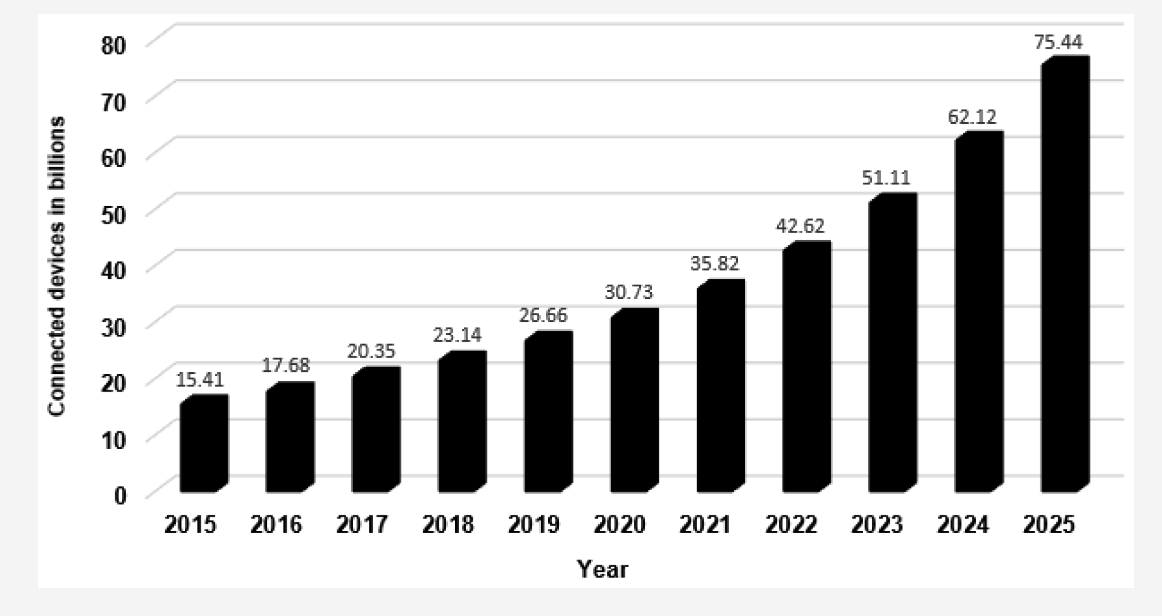
\includegraphics[width=1\textwidth]{figures/number_of_iot.png}
    \caption{The growth of IoT devices from 2015 to 2025 ref(img1)}
    \label{fig:num_of_iot}
\end{figure}


We would like to mention a number of common characteristics that most IoT devices share: 

\begin{itemize}
    \item Connectivity - with the help of a number of protocols they can communicat with each other.
    \item Heterogeneity: a variety of devices and objects including communication protocols
    \item Unique identity: a unique identifier for each device 
    \item Big data: IoT number one source of big data 
\end{itemize}

However IoT suffers from its typical architecture design which is the centralized architecture. These centralized server either on the cloud or on premise manages and deals with all requests coming from various nodes. This architecture comes with multiple challenges: scalability issues, security and privacy challenges and issues with the analysis of big data (ref130). 

\subsection{Enabling Deep Learning in IoT}
AI has become a buzzword and one of the topics that has a significant impact on many different domains. In Figure~\ref{fig:ai_terms} depicts the relationship between Artificial Intelligence, Machine Learning and Deep Learning. In simple words AI encapsulates the imitation of human intelligence by computers. Machine learning is the technique used to allow computer programs to access data and use it to automatically learn and improve from experience. The neural network involves a large number of processors operating in parallel arranged in tiers , in the same way neurons in our brain works. While deep learning employees neural networks but with many layers of neural networks. 


\begin{figure}[!htb]
    \centering
    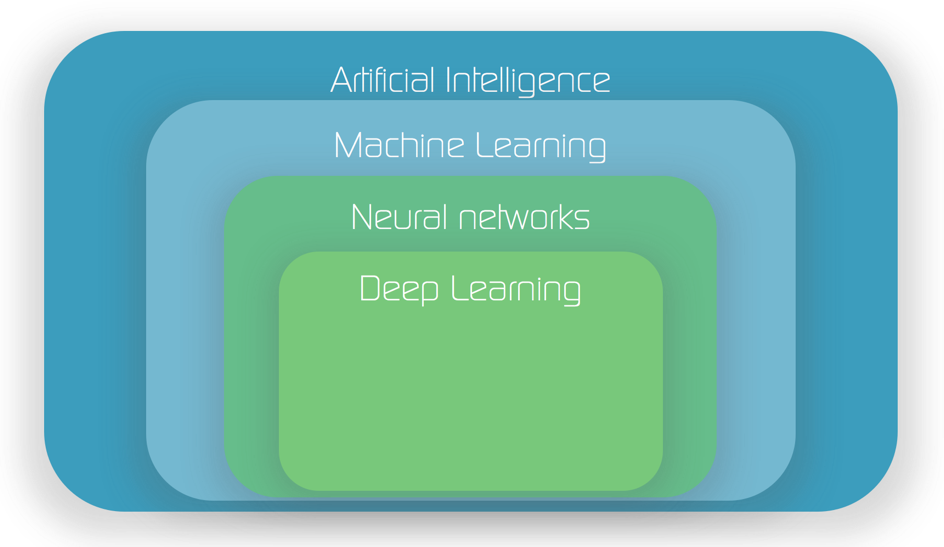
\includegraphics[width=1\textwidth]{figures/ai_classification.png}
    \caption{Relationship of AI terms.(refimg12)}
    \label{fig:ai_terms}
\end{figure}
We already know that AI can solve and make sense of the immense amount of data produced from IoT devices. However the main question for research appears “How to deploy neural networks directly on these tiny devices? Therefore there is an opportunity and challenge at the same time to run machine learning on such tiny IoT devices based on microcontrollers. By running machine learning on these tiny devices, we can directly perform real time data analytics in the device itself, therefore avoiding the need to store all the data generated from the IoT device. Typically commercial use cases of smart IoT devices often offload the Artificial Intelligence part to the cloud. 
One of the most recent study(ref321) that worked on this direction tested two approaches with deep learning: 
\begin{itemize}
    \item Offloading deep learning platforms to the cloud
    \item Migrate deep learning to an IoT device
\end{itemize}

The two approaches were tested and look from two different perspectives,  whether offloading machine learning can reduce energy efficiency and satisfy the real time requirements of object recognition. 
In the first approach they used convolutional neural networks on the cloud, while the Jetson TX1 was responsible to just take images and forward them to the cloud. The results show that executing machine learning in the Jetson TX1 consumed more energy compared to the offloading to the cloud. However offloading AI to the cloud also comes with drawbacks, it has lead to a range of latency starting from 2 seconds that goes up to 5 seconds which is far higher compare to the execution of AI in the Jetson TX1 itself. This leads to conclude that the variability of response time make it quite unreliable and not useful for real time AI processing. 

Furthermore MIT researchers ref(mit123) have implemented a sytem called MCUNet, which has a high potential to bring deep learning in much smaller devices like tiny computer chips despite their limited memory and computational power. 

\subsection{Intersection of Blockchain and AI}

There is a high research on Blockchain and AI but analysed in isolation and in various domains and applications. Some research ref(17) focus on the application of AI in the Blockchain for making blockchain more efficient for instance, consensus mechanisms and better governance. However there seem to be more research and applications of Blockchain in AI. Similar to IoT, AI domain also suffers from security, its centralized architecture and resource limitations. This is exactly what blockchain is looking to solve. There is a lot of discussion and research in this area, however most of them are reviews and solutions that do not provide a use case or implement such solutions. In order to have a global image the Table ref() describes the features of the two technologies and the benefits of integrating such features.

There is another interesting contribution (ref) that came up with an AI blockchain platform to fight the propagation of fake news. This platform allows publishers to setup a distribution platform in the blockchain while AI will be monitoring on the actors who are adding news to the blockchain. Expectation is that the blockchain will server as the "factual database" to trace back the news. So the news which cannot be traced back to the blockchain will be automatically considered fake. 




\begin{table}[hbt!]

    
    \begin{tabular}{  p{4.4cm}  p{4.4cm}  p{5.4cm} }
      
\textbf{Blockchain}      
& \textbf{AI}   
& \textbf{Benefits of blockchain} \\\midrule
Decentralized & Centralized        
& Enhanced Data Security \\\hline

Immutable & Probabilistic       
& Collective Decision making \\\hline


Data Integrity & Volatile      
& Decentralized Intelligence \\\hline

Resilient to attacks & Data, knowledge and decision centric     
& High Efficiency \\\hline

Deterministic  &
Changing      
& Improved trust on robotics decision \\
        \bottomrule
    \end{tabular}
    \caption{Benefits of integrating blockchain into AI  (adopted from \ldots%\citealt{crouch2012doing}
    )}
    \label{crouch}
\end{table}

\subsection{Integration of Blockchain with IoT}

We have already listed a number of issues that IoT world is facing, which mainly is the centraized architecture, security and privacy. Therefore pretty much of the research is focused in this area, typically with the advantages of blockchain those gaps can be closed. For instance ref(IS) attempted to discover the security gaps that could be mitigated with the help of the blockchain to ensure the reliability and availability of the data.

Other studies (refIS) attempted to integrate crypto based blockchains such as Ethereum in their approaches. We argue here that most of the crypto based blockchains are not efficient in storing data coming from IoT devices. First users have to pay fees for each transactions and the there is a limitation in the number of transactions it can process. Although we can escape from the centralization still there is the risk of bottleneck. Therefore in our study we will be using Hyperledger Fabric a non crypto based blockchain aimed for storing data. 


































\begin{comment}

\begin{table}[!h]
\definecolor{LightCyan}{rgb}{0.88,1,1}
\definecolor{Gray}{gray}{0.9}
\newcolumntype{g}{>{\columncolor{LightCyan}}c}
\noindent\begin{tabularx}{\textwidth}{|g|l|X|}

\hline apple  & StackOverflow & Dardh \\
\hline 
\begin{itemize}
\item[--] Decentralized

\item[--] Deterministic
\item[--] Immutable
\item[--] Data Integrity

\end{itemize}

& StackOverflow &
 lots of long text. lots of long text. lots of long text. lots of long text. lots of long text. \\
\hline 

\end{tabularx}
\caption{Truth Tables and Accuracy Measures for each modeling library.}
    \label{tab:truthTables}

 \end{table}



\end{comment}

 
 
 
 \section{Use cases on AI, IoT and Blockchain}
 
 We have already described the intersections on how Blockchain, AI and IoT accommodate each other in pair, however there is a very high potential for the usage of all the three domains in one use case. With such a high number of IoT devices there is a potential to take the advantage of AI and Blockchain at the same time. Based on reforacle, every institution  which will take the advantage of exploiting these technologies, it will have the chance to radically enhance their existing processes and create entirely new business models. 
 
An interesting work ref(smartcity)  presents how the collaboration of the three domains can build a sustainable smart city. Given the many issues people in urban areas face, the concept of the sustainable smart city brings new opportunities for the application. With their new approach they aim to have a transparent monitoring system for measuring pollution which in turn will help raise awareness to the population. 

In another use case the authors (refhomeauto) propose an IoT based home automation and surveillance system. In this setup they have employed a raspberry pi, a camera attached to it and a DC motor for controlling the door. The video surveillance is not detecting or recognizing people, so the burden falls into the owner who through the help of a front end will be able to open the door. Therefore compare to our solution there is no AI and blockchain integrated. 


A use case that pretty much is matching with our use case is a design and implementation of a camera based sensor for room capacity monitoring. The aim of it is to count the number of people present in a room with the help of a raspberry pi and a camera. In Figure~\ref{fig:raum} we can see the architectural overview. 

\begin{figure}[!htb]
    \centering
    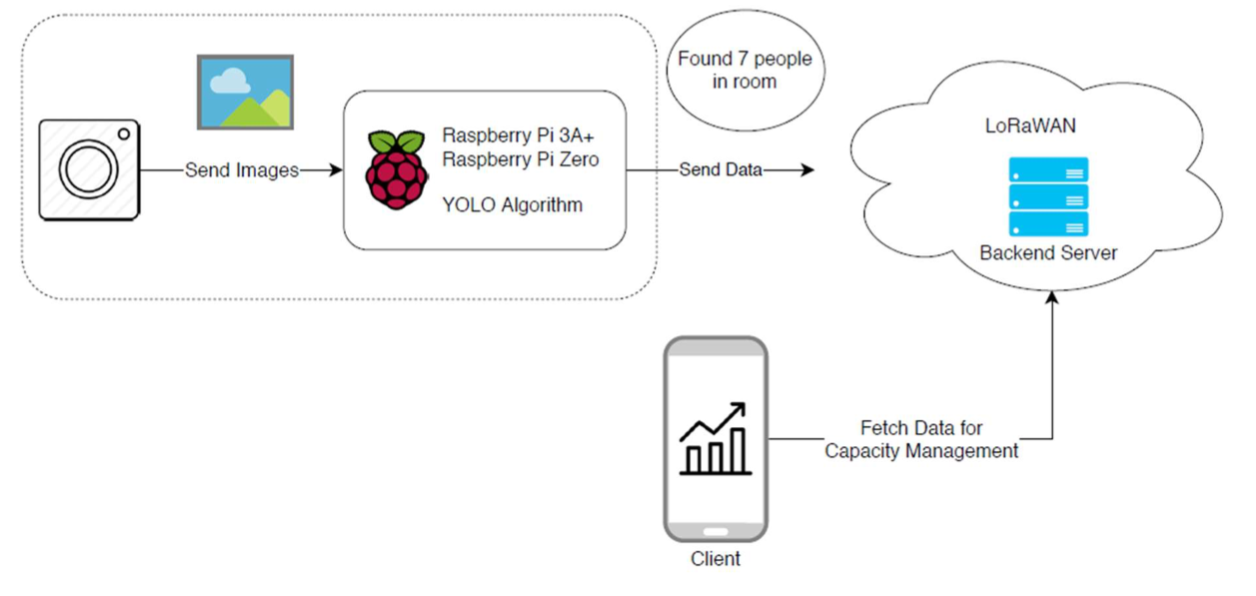
\includegraphics[width=1\textwidth]{figures/raumbelegung.png}
    \caption{Architectural Overview(ref)}
    \label{fig:raum}
\end{figure}

Their architecture employees AI and IoT. This use case was designed and implemented by a group of students at FHNWS who employed a raspberry pi equipped with camera and lora gateway. The role of camera is to just take pictures and after that some machine learning algorithm will analyze the image and find the number of people in the room. Once done the data is then send to a LoraWan Server. To achieve that they have attached a LoraWan antenna to the RPI and eventually with a front end they can monitor the room. So face detection happens in the RPI, the algorithm counts the number of people in the image and sends it to the Lorawan Backend Server. From here we can conclude that the issue of centralisation is still open, data is being stored in a database, security issues are not tackled enough. Besides there is also the need for a RPI to be placed in a room as the camera is attached to it and that needs power to run. 

With out proposed architecture we are not only going automate the IoT-based surveillance system but provide a robust solution that will take care of the leaks that AI and blockchain will be able to neutralize. 


\chapter{Face Detection and Recognition}
\label{chap:face_detection}




